%%%%%%%%%%%%%%%%%%%%%%%%%%%%%%%%%%%%%%%%%%%%%%%%%%%%%%%%
%%
\chapter{The Recipes}
\label{ch:the_recipes}
%%
%%%%%%%%%%%%%%%%%%%%%%%%%%%%%%%%%%%%%%%%%%%%%%%%%%%%%%%%


%%%%%%%%%%%%%%%%%%%%%%%%%%%%%%%%%%%%%%%%%%%%%%%%%%%%%%%%
%%
\clearpage
\newpage
\section{The cal\_DARK recipe}
\label{ch:the_recipes:cal_DARK_spirou}
%%
%%%%%%%%%%%%%%%%%%%%%%%%%%%%%%%%%%%%%%%%%%%%%%%%%%%%%%%%

Dark with short exposure time (~5min, to be defined during AT-4) to check if read-out noise, dark current and hot pixel mask are consistent with the ones obtained during technical night. Quality control is done automaticaly by the pipeline (see Section \ref{section:qc_cal_DARK_spirou}). \\


% -------------------------------------------------------
\subsection{The inputs}
% -------------------------------------------------------
The input of \calDARK is as follows:
\begin{cmdbox}
cal_DARK_spirou.py  night_repository  filenames
\end{cmdbox}
\noindent or
\begin{pythonbox}
import cal_DARK_spirou
night_reposityory = '20170710'
filenames = ['dark_dark02d406.fits']
cal_DARK_spirou.main(night_repository, filenames)
\end{pythonbox}

\noindent where `night\_repository' defines \argnightname and `filenames' define the list of files in \argfilenames. All files in filenames must be valid python strings separated by a space (command line) or in a line (python). \\

\noindent Filename prefixes allowed are:
\begin{itemize}
	\item dark\_dark
\end{itemize}

% -------------------------------------------------------
\subsection{The outputs}
% -------------------------------------------------------
The outputs of \calDARK are as follows:

\begin{itemize}
\item \definevariable{text:darkfile}{darkfile} in form:
\begin{tcustomdir}
\{\reduceddir\}\{date prefix\}\_\{file\}.fits
\end{tcustomdir}

\item \definevariable{text:darkbadpixfile}{darkbadpixfile} in form:
\begin{tcustomdir}
\{\reduceddir\}\{date prefix\}\_\{file\}\_badpixel.fits
\end{tcustomdir}
\end{itemize}

\noindent where `date prefix' is constructed from \argnightname and the file name is the first file in \argfilenames.

% -------------------------------------------------------
\subsection{Summary of procedure}
% -------------------------------------------------------
\begin{enumerate}
\item adds defined `dark\_dark' files together
\item resizes the image
\item calculates the fraction of dead pixels [full, blue part, red part]
\item calculates median dark level [full, blue part, red part]
\item calculates threshold of dark level to retain
\item removes dead pixels by setting them to 0
\item does some quality control
\item updates calibDB with key "DARK"
\end{enumerate}


% -------------------------------------------------------
\subsection{Quality Control}
% -------------------------------------------------------


There are currently three quality control checks for cal\_DARK\_spirou
\begin{itemize}
\item Unexpected median dark level if: 
\begin{thighlight}
\begin{equation}
\text{Median Flux} > \text{\definevariable{text:qc_max_darklevel}{qc\_max\_darklevel}}
\end{equation}
\end{thighlight}

\item Unexpected fraction of dead pixels if: 
\begin{thighlight}
\begin{equation}
\text{Number of dead pixels} > \text{\definevariable{text:qc_max_dead}{qc\_max\_dead}}
\end{equation}
\end{thighlight}

\item Unexpected fraction of dark pixels if:
\begin{thighlight}
\begin{equation}
\text{Number of bad dark pixels} > \text{\definevariable{text:qc_max_dark}{qc\_max\_dark}}
\end{equation}
\end{thighlight}
\end{itemize}

If none of these quality control criteria are valid then the output file is passed into the \calibdb with key `DARK' for the `darkfile' and `BADPIX' for the `darkbadpixfile'.

% -------------------------------------------------------
\newpage
\subsection{Example working run}
% -------------------------------------------------------

An example run where everything worked is below:

\begin{cmdboxprintspecial}
@g20:57:30.8 -   || ***************************************** 
20:57:30.8 -   || * SPIROU \@(#) Geneva Observatory (0.0.057) 
20:57:30.8 -   || ***************************************** 
20:57:30.8 -   ||(dir_data_raw)      DRS_DATA_RAW=/scratch/Projects/spirou_py3/data/raw 
20:57:30.8 -   ||(dir_data_reduc)    DRS_DATA_REDUC=/scratch/Projects/spirou_py3/data/reduced 
20:57:30.8 -   ||(dir_calib_db)      DRS_CALIB_DB=/scratch/Projects/spirou_py3/data/calibDB 
20:57:30.8 -   ||(dir_data_msg)      DRS_DATA_MSG=/scratch/Projects/spirou_py3/data/msg 
20:57:30.8 -   ||(print_level)       PRINT_LEVEL=all         %(error/warning/info/all) 
20:57:30.8 -   ||(log_level)         LOG_LEVEL=all         %(error/warning/info/all) 
20:57:30.8 -   ||(plot_graph)        DRS_PLOT=1            %(def/undef/trigger) 
20:57:30.8 -   ||(used_date)         DRS_USED_DATE=undefined
20:57:30.8 -   ||(working_dir)       DRS_DATA_WORKING=/scratch/Projects/spirou_py3/data/tmp/
20:57:30.8 -   ||                    DRS_INTERACTIVE is not set, running on-line mode
20:57:30.8 -   ||                    DRS_DEBUG is set, debug mode level:1
20:57:30.8 -   |ipython:2d406|Now running : ipython on file(s): dark_dark02d406.fits
20:57:30.8 -   |ipython:2d406|On directory /scratch/Projects/spirou_py3/data/raw/20170710
20:57:30.8 -   |ipython:2d406|ICDP_NAME loaded from: /scratch/Projects/spirou_py3/INTROOT/config/constants_SPIROU.py
20:57:30.8 - * |ipython:2d406|Correct type of image for dark (dark_dark)
20:57:31.0 - * |ipython:2d406|Now processing Image TYPE UNKNOWN with ipython recipe
20:57:31.0 -   |ipython:2d406|Reading Image /scratch/Projects/spirou_py3/data/raw/20170710/dark_dark02d406.fits
20:57:31.0 -   |ipython:2d406|Image 2048 x 2048 loaded
20:57:31.0 - * |ipython:2d406|Dark Time = 597.489 s
20:57:31.2 -   |ipython:2d406|Doing Dark measurement
20:57:31.5 - * |ipython:2d406|In Whole det: Frac dead pixels= 14.7 % - Median= 0.35 ADU/s - Percent[5:95]= 0.08-99.57 ADU/s
20:57:31.5 - * |ipython:2d406|In Blue part: Frac dead pixels= 1.0 % - Median= 0.15 ADU/s - Percent[5:95]= 0.09-0.53 ADU/s
20:57:31.5 - * |ipython:2d406|In Red part : Frac dead pixels= 20.5 % - Median= 2.11 ADU/s - Percent[5:95]= 0.18-232.09 ADU/s
20:57:31.5 - * |ipython:2d406|Frac pixels with DARK > 100.0 ADU/s = 4.3 %
@g@y20:57:31.6 - \@ |python warning|Line 138 warning reads: invalid value encountered in greater
@y@g20:57:31.6 - * |ipython:2d406|Total Frac dead pixels (N.A.N) + DARK > 100.0 ADU/s = 18.9 %
20:57:32.1 - * |ipython:2d406|QUALITY CONTROL SUCCESSFUL - Well Done -
20:57:32.1 -   |ipython:2d406|Saving Dark frame in 20170710_dark_dark02d406.fits
@g@y20:57:32.4 - \@ |python warning|Line 980 warning reads: Card is too long, comment will be truncated.
@y@g20:57:32.4 -   |ipython:2d406|Saving Bad Pixel Map in 20170710_dark_dark02d406_badpixel.fits
@g@y20:57:32.7 - \@ |python warning|Line 980 warning reads: Card is too long, comment will be truncated.
@y@g20:57:32.7 - * |ipython:2d406|Updating Calib Data Base with DARK
20:57:32.7 - * |ipython:2d406|Updating Calib Data Base with BADPIX
20:57:32.7 - * |ipython:2d406|Recipe ipython has been succesfully completed
@g
\end{cmdboxprintspecial}


% -------------------------------------------------------
\newpage
\subsection{Interactive mode}
% -------------------------------------------------------


\noindent In interactive mode (\definevariable{text:drs_plot}{DRS\_PLOT} = 1) three figures will also appear (see Figure \ref{figure:cal_DARK_spirou}).


\begin{figure}

\begin{center}
\begin{minipage}{.495\textwidth}
\begin{center}
\includegraphics[width=\textwidth]{Figures/cal_DARK_spirou_1.pdf}
a
\end{center}
\end{minipage}%
\begin{minipage}{.495\textwidth}
\begin{center}
\includegraphics[width=\textwidth]{Figures/cal_DARK_spirou_2.pdf}
b
\end{center}
\end{minipage}%
\end{center}

\begin{center}
\begin{minipage}{.495\textwidth}
\begin{center}
\includegraphics[width=\textwidth]{Figures/cal_DARK_spirou_3.pdf}
c
\end{center}
\end{minipage}%
\end{center}

\caption{\textbf{(a)} The image with overplot red and blue regions (red/blue rectangles). \textbf{(b)} The bad pixel mask, bad pixels have a value=1 (in black) and good pixels have a value=0 (in white). \textbf{(c)} Histograms of the image regions, the full image (in green), the blue section (in blue) and the red section (in red). \label{figure:cal_DARK_spirou}}
\end{figure}



%%%%%%%%%%%%%%%%%%%%%%%%%%%%%%%%%%%%%%%%%%%%%%%%%%%%%%%%
%%
\clearpage
\newpage
\section{The cal\_BADPIX recipe}
\label{ch:the_recipes:cal_loc_RAW_spirou}
%%
%%%%%%%%%%%%%%%%%%%%%%%%%%%%%%%%%%%%%%%%%%%%%%%%%%%%%%%%

Recipe to generate the bad pixel map. \\

% -------------------------------------------------------
\subsection{The inputs}
% -------------------------------------------------------
The input of \calbadpix is as follows:
\begin{cmdbox}
cal_BADPIX_spirou.py  night_repository  flatfile, darkfile
\end{cmdbox}
\noindent or
\begin{pythonbox}
import cal_DARK_spirou
night_reposityory = '20170710'
darkfile = 'dark_dark02d406.fits'
flatfile = 'flat_flat02f10.fits'
cal_DARK_spirou.main(night_repository, flatfile=flatfile, darkfile=darkfile)
\end{pythonbox}

\noindent where `night\_repository' defines \argnightname and `filenames' define the list of files in \argfilenames. All files in filenames must be valid python strings separated by a space (command line) or in a line (python) and must have the folowing prefixes:
\noindent File prefixes allowed:
\begin{itemize}
	\item flat\_flat (flatfile)
	\item dark\_dark (darkfile)
\end{itemize}

% % -------------------------------------------------------
% \subsection{The outputs}
% % -------------------------------------------------------

% The outputs of \definevariable{text:badpixelfits}{badpixelfits} are as follows:

% \begin{itemize}
% \item {badpixelfits} in form:
% \begin{tcustomdir}
% \{\reduceddir\}\{date prefix\}\_\{file\}\_badpixelfits.fits
% \end{tcustomdir}
% \end{itemize}

% \noindent where `date prefix' is constructed from \argnightname and the file name is the first file in \argfilenames.

% % -------------------------------------------------------
% \subsection{Summary of procedure}
% % -------------------------------------------------------
% \begin{enumerate}
% \item {}
% \end{enumerate}


% % -------------------------------------------------------
% \subsection{Quality Control}
% % -------------------------------------------------------

% There are currently three quality control checks for cal\_DARK\_spirou
% \begin{itemize}
% \item Unexpected {} if: 
% 	\begin{equation}
	
% 	\end{equation}

% \end{itemize}

% If none of these quality control criteria are valid then the output file is passed into the \calibdb with key `{}'.


% % -------------------------------------------------------
% \newpage
% \subsection{Example working run}
% % -------------------------------------------------------

% An example run where everything worked is below:

% \begin{cmdboxprintspecial}
% @g

% @g
% \end{cmdboxprintspecial}


% % -------------------------------------------------------
% \newpage
% \subsection{Interactive mode}
% % -------------------------------------------------------


% \noindent In interactive mode (\definevariable{text:drs_plot}{DRS\_PLOT} = 1) three figures will also appear (see Figure \ref{figure:}).


% \begin{figure}

% \begin{center}
% \begin{minipage}{.495\textwidth}
% \begin{center}
% \includegraphics[width=\textwidth]{Figures/cal_DARK_spirou_1.pdf}
% a
% \end{center}
% \end{minipage}%
% \begin{minipage}{.495\textwidth}
% \begin{center}
% \includegraphics[width=\textwidth]{Figures/cal_DARK_spirou_2.pdf}
% b
% \end{center}
% \end{minipage}%
% \end{center}

% \begin{center}
% \begin{minipage}{.495\textwidth}
% \begin{center}
% \includegraphics[width=\textwidth]{Figures/cal_DARK_spirou_3.pdf}
% c
% \end{center}
% \end{minipage}%
% \end{center}

% \caption{\textbf{(a)} The image with overplot red and blue regions (red/blue rectangles). \textbf{(b)} The bad pixel mask, bad pixels have a value=1 (in black) and good pixels have a value=0 (in white). \textbf{(c)} Histograms of the image regions, the full image (in green), the blue section (in blue) and the red section (in red). \label{figure:cal_DARK_spirou}}
% \end{figure}

%%%%%%%%%%%%%%%%%%%%%%%%%%%%%%%%%%%%%%%%%%%%%%%%%%%%%%%%
%%
\clearpage
\newpage
\section{The cal\_loc recipe}
\label{ch:the_recipes:cal_loc_RAW_spirou}
%%
%%%%%%%%%%%%%%%%%%%%%%%%%%%%%%%%%%%%%%%%%%%%%%%%%%%%%%%%

Locates the orders on the `dark\_flat' or `flat\_dark' images.\\

% % -------------------------------------------------------
% \subsection{The inputs}
% % -------------------------------------------------------
% The input of {\_} is as follows:
% \begin{cmdbox}

% \end{cmdbox}
% \noindent or
% \begin{pythonbox}
% import 

% cal_DARK_spirou.main()
% \end{pythonbox}

% \noindent where `night\_repository' defines \argnightname and `filenames' define the list of files in \argfilenames. All files in filenames must be valid python strings separated by a space (command line) or in a line (python) and must have the folowing prefixes:
% \noindent File prefixes allowed:
% \begin{itemize}
% 	\item {}
% \end{itemize}

% % -------------------------------------------------------
% \subsection{The outputs}
% % -------------------------------------------------------
% The outputs of \definevariable{}{} are as follows:

% \begin{itemize}
% \item {} in form:
% \begin{tcustomdir}
% \{\reduceddir\}\{date prefix\}\_\{file\}.fits
% \end{tcustomdir}
% \end{itemize}

% \noindent where `date prefix' is constructed from \argnightname and the file name is the first file in \argfilenames.

% % -------------------------------------------------------
% \subsection{Summary of procedure}
% % -------------------------------------------------------
% \begin{enumerate}
% \item {}
% \end{enumerate}


% % -------------------------------------------------------
% \newpage
% \subsection{Example working run}
% % -------------------------------------------------------

% An example run where everything worked is below:

% \begin{cmdboxprintspecial}
% @g

% @g
% \end{cmdboxprintspecial}


% % -------------------------------------------------------
% \newpage
% \subsection{Interactive mode}
% % -------------------------------------------------------


% \noindent In interactive mode (\definevariable{text:drs_plot}{DRS\_PLOT} = 1) three figures will also appear (eee figures \ref{figure:cal_DARK_spirou_1}, \ref{figure:cal_DARK_spirou_2}, and \ref{figure:cal_DARK_spirou_3}).

% \begin{figure}
% \begin{center}
% \includegraphics[width=.8\textwidth]{}
% \caption{ \label{figure:1}}
% \end{center}
% \end{figure}







%%%%%%%%%%%%%%%%%%%%%%%%%%%%%%%%%%%%%%%%%%%%%%%%%%%%%%%%
%%
\clearpage
\newpage
\section{The cal\_SLIT recipe}
\label{ch:the_recipes:cal_SLIT_spirou}
%%
%%%%%%%%%%%%%%%%%%%%%%%%%%%%%%%%%%%%%%%%%%%%%%%%%%%%%%%%



% % -------------------------------------------------------
% \subsection{The inputs}
% % -------------------------------------------------------
% The input of {\_} is as follows:
% \begin{cmdbox}

% \end{cmdbox}
% \noindent or
% \begin{pythonbox}
% import 

% cal_DARK_spirou.main()
% \end{pythonbox}

% \noindent where `night\_repository' defines \argnightname and `filenames' define the list of files in \argfilenames. All files in filenames must be valid python strings separated by a space (command line) or in a line (python) and must have the folowing prefixes:
% \noindent File prefixes allowed:
% \begin{itemize}
% 	\item {}
% \end{itemize}

% % -------------------------------------------------------
% \subsection{The outputs}
% % -------------------------------------------------------
% The outputs of \definevariable{}{} are as follows:

% \begin{itemize}
% \item {} in form:
% \begin{tcustomdir}
% \{\reduceddir\}\{date prefix\}\_\{file\}.fits
% \end{tcustomdir}

% \noindent where `date prefix' is constructed from \argnightname and the file name is the first file in \argfilenames.

% % -------------------------------------------------------
% \subsection{Summary of procedure}
% % -------------------------------------------------------
% \begin{enumerate}
% \item {}
% \end{enumerate}


% % -------------------------------------------------------
% \newpage
% \subsection{Example working run}
% % -------------------------------------------------------

% An example run where everything worked is below:

% \begin{cmdboxprintspecial}
% @g

% @g
% \end{cmdboxprintspecial}


% % -------------------------------------------------------
% \newpage
% \subsection{Interactive mode}
% % -------------------------------------------------------

% \noindent In interactive mode three figures will also appear (see Figure \ref{figure:}).

% \begin{figure}

% \begin{center}
% \begin{minipage}{.495\textwidth}
% \begin{center}
% \includegraphics[width=\textwidth]{Figures/cal_DARK_spirou_1.pdf}
% a
% \end{center}
% \end{minipage}%
% \begin{minipage}{.495\textwidth}
% \begin{center}
% \includegraphics[width=\textwidth]{Figures/cal_DARK_spirou_2.pdf}
% b
% \end{center}
% \end{minipage}%
% \end{center}

% \begin{center}
% \begin{minipage}{.495\textwidth}
% \begin{center}
% \includegraphics[width=\textwidth]{Figures/cal_DARK_spirou_3.pdf}
% c
% \end{center}
% \end{minipage}%
% \end{center}

% \caption{\textbf{(a)} The image with overplot red and blue regions (red/blue rectangles). \textbf{(b)} The bad pixel mask, bad pixels have a value=1 (in black) and good pixels have a value=0 (in white). \textbf{(c)} Histograms of the image regions, the full image (in green), the blue section (in blue) and the red section (in red). \label{figure:cal_DARK_spirou}}
% \end{figure}


%%%%%%%%%%%%%%%%%%%%%%%%%%%%%%%%%%%%%%%%%%%%%%%%%%%%%%%%
%%
\clearpage
\newpage
\section{The cal\_FF recipe}
\label{ch:the_recipes:cal_FF_RAW_spirou}
%%
%%%%%%%%%%%%%%%%%%%%%%%%%%%%%%%%%%%%%%%%%%%%%%%%%%%%%%%%




%%%%%%%%%%%%%%%%%%%%%%%%%%%%%%%%%%%%%%%%%%%%%%%%%%%%%%%%
%%
\clearpage
\newpage
\section{The cal\_extract recipes}
\label{ch:the_recipes:cal_extract_RAW_spirou}
%%
%%%%%%%%%%%%%%%%%%%%%%%%%%%%%%%%%%%%%%%%%%%%%%%%%%%%%%%%







%%%%%%%%%%%%%%%%%%%%%%%%%%%%%%%%%%%%%%%%%%%%%%%%%%%%%%%%
%%
\clearpage
\newpage
\section{The cal\_DRIFT recipes}
\label{ch:the_recipes:cal_DRIFT_RAW_spirou}
%%
%%%%%%%%%%%%%%%%%%%%%%%%%%%%%%%%%%%%%%%%%%%%%%%%%%%%%%%%






%%%%%%%%%%%%%%%%%%%%%%%%%%%%%%%%%%%%%%%%%%%%%%%%%%%%%%%%
%%
\clearpage
\newpage
\section{The cal\_BADPIX recipe}
\label{ch:the_recipes:cal_BADPIX_spirou}
%%
%%%%%%%%%%%%%%%%%%%%%%%%%%%%%%%%%%%%%%%%%%%%%%%%%%%%%%%%




%%%%%%%%%%%%%%%%%%%%%%%%%%%%%%%%%%%%%%%%%%%%%%%%%%%%%%%%
%%
\clearpage
\newpage
\section{The cal\_HC recipe}
\label{ch:the_recipes:cal_HC_E2DS_spirou}
%%
%%%%%%%%%%%%%%%%%%%%%%%%%%%%%%%%%%%%%%%%%%%%%%%%%%%%%%%%



%%%%%%%%%%%%%%%%%%%%%%%%%%%%%%%%%%%%%%%%%%%%%%%%%%%%%%%%
%%
\clearpage
\newpage
\section{The cal\_WAVE recipe}
\label{ch:the_recipes:cal_WAVE_E2DS_spirou}
%%
%%%%%%%%%%%%%%%%%%%%%%%%%%%%%%%%%%%%%%%%%%%%%%%%%%%%%%%%



%%%%%%%%%%%%%%%%%%%%%%%%%%%%%%%%%%%%%%%%%%%%%%%%%%%%%%%%
%%
\clearpage
\newpage
\section{The cal\_CCF recipe}
\label{ch:the_recipes:cal_CCF_E2DS_spirou}
%%
%%%%%%%%%%%%%%%%%%%%%%%%%%%%%%%%%%%%%%%%%%%%%%%%%%%%%%%%


%%%%%%%%%%%%%%%%%%%%%%%%%%%%%%%%%%%%%%%%%%%%%%%%%%%%%%%%
%%
\clearpage
\newpage
\section{The pol\_spirou recipe}
\label{ch:the_recipes:pol_spirou}
%%
%%%%%%%%%%%%%%%%%%%%%%%%%%%%%%%%%%%%%%%%%%%%%%%%%%%%%%%%


%%%%%%%%%%%%%%%%%%%%%%%%%%%%%%%%%%%%%%%%%%%%%%%%%%%%%%%%
%%
\clearpage
\newpage
\section{The validation recipes recipe}
\label{ch:the_recipes:cal_validate_spirou}
%%
%%%%%%%%%%%%%%%%%%%%%%%%%%%%%%%%%%%%%%%%%%%%%%%%%%%%%%%%